\documentclass[conference]{IEEEtran}

% Eingabecodierung
\usepackage[utf8]{inputenc}

% Sprachraum
\usepackage[ngerman]{babel}

% Schriftcodierung Europäische Zeichen
\usepackage[T1]{fontenc}

% Schrifteinstellungen
% Vektorschrift
\usepackage{lmodern}
% Serifenlose Schrift 
\renewcommand{\familydefault}{\sfdefault}
% Mathe-Schrift ohne Serifen 
\usepackage{sansmath}
% aktiviert serifenlose Matheschrift  	
\sansmath
% harmonische Typenverteilung 							
\usepackage{microtype}	

% Literatur einbinden
% https://tex.stackexchange.com/questions/308326/latex-bibtex-throws-3-errors
\usepackage[babel, german=quotes]{csquotes}
\usepackage[
backend=bibtex, 
style=numeric-comp,
block=ragged,			
sorting=none,			
]{biblatex}
\addbibresource{TPM.bib}

% Mathemodus
\usepackage{amsmath,amssymb}

% Bilder einbinden
\usepackage{graphicx}
\graphicspath{{images/}}

% Code einbinden
\usepackage{listings}

% Grafiken zeichen
\usepackage{tikz}
\usetikzlibrary{calc,arrows,positioning} 

% Zum automatischen und manuellen Erstellung von dynamischen Querverweisen in Dokumenten
\usepackage{hyperref}
\hypersetup{
colorlinks,
citecolor=black,
filecolor=black,
linkcolor=black,
urlcolor=black
}

\begin{document}

% makes the title
\title{Umgehung von Festplattenverschlüsselung mit Trusted Platform Module am Beispiel von BitLocker\\}

% make the author
\author{
	\IEEEauthorblockA{
		\textit{0xffd700}\\
		\textit{-}\\
		\textit{-} \\
		\textit{-} \\
		\line(1,0){450} \\
	}
}

\maketitle

%Zusammenfassung
\begin{abstract}
	Persönliche und betriebliche Daten sind dank Laptops und portablen Datenspeichergeräten immer und überall abrufbar. Die Bequemlichkeit des ständigen physikalischen Zugangs bringt jedoch auch viele Sicherheitsrisiken. Im Rahmen dieser Arbeit betrachten wir die Schutzmöglichkeit von Daten anhand einer Festplattenverschlüsselung. Es wird die grundlegende Funktionsweise der Festplattenverschlüsselung besonders in Kombination mit Trusted Platform Modules (TPM) vorgestellt und bereits bekannte Möglichkeiten der Umgehung aufgezeigt. Anhand BitLocker, der Festplattenverschlüsselungslösung von Microsoft, wird ein Angriffsszenario nachgestellt. In diesem wird die unverschlüsselte Kommunikation zwischen BitLocker und dem TPM genutzt, um zur Entschlüsselung relevante Daten abzufangen. Die Durchführbarkeit wird anhand eines praktischen Versuchs bewiesen und unter den Aspekten eines realistischen Angriffsszenarios evaluiert. Der Versuchsaufbau belegt, dass Festplattenverschlüsselungen, welche nur durch TPMs verifiziert werden, nur begrenzt vor Datendiebstahl schützen und zeigt Möglichkeiten der Prävention durch zusätzliche Benutzerauthentifizierung. \\
\end{abstract}

%Index Terms

\begin{IEEEkeywords}
	Trusted Platform Module, BitLocker, Festplattenverschlüsselung
\end{IEEEkeywords}

\section{Einleitung}
Während in der Vergangenheit Computer vor allem in Privat- und Büroräumen standen, nimmt der Einsatz von mobilen Geräten immer weiter zu. Ob in der Bahn das morgendliche Meeting vorbereitet wird oder der Student seine wissenschaftliche Arbeit zur Abwechslung in einem Café schreibt. Diese mobile Datenhaltung ist nicht nur für die Nutzer bequem, sondern erleichtert auch Hackern den Arbeitsalltag. Der sicherheitsbewusste Hardwarebesitzer oder Firmeninhaber setzt auf eine Festplattenverschlüsselung, die dem Angreifer bei physikalischem Zugang das direkte Auslesen der Daten verhindert. Dieser Schutzmechanismus hat sich bewährt und wird bei vielen Computerherstellern durch einen kryptografischen Chip, das sogenannte Trusted Platform Module, unterstützt. Im Rahmen dieser Arbeit wird die Sicherheit von Festplattenverschlüsselung am Beispiel der von Microsoft entwickelten Software BitLocker in Kombination mit einem TPM überprüft. Dabei wird getestet ob ein TPM ohne weitere Benutzerauthentifizierung genug Schutz bietet und auf die Möglichkeit der Umsetzung in einem zeitlich und durch Ressourcen begrenzten Szenario eingegangen. 

\section{Festplattenverschlüsselung}
Festplattenverschlüsselung ist eine Methode zum Schutz von Daten gegen physikalische Angriffe durch Verschlüsselung des gesamten Datenträgers oder einzelner Sektoren. Ohne diese Sicherheitsmaßnahme können Datenträger aus einem Gerät entnommen werden und unter Verwendung eines entsprechenden Adapters an ein anderes System angeschlossen werden. Dies ermöglicht eine Einsichtnahme aller darauf gespeicherter Daten. \cite{SibingerChristophANDMullerTilo.2014}

\subsection{Trusted Platform Module}
Trusted Platform Modules wurden entwickelt, um den Sicherheitsstandard von Systemen, die historisch meist softwarebasiert waren, durch eine weitere Hardwarekomponente zu ergänzen. In den meisten Systemen als Coprozessorchip auf dem Mainboard realisiert, wird TPM zum Ausführen kryptografischer Operationen genutzt. Diese umfassen das Generieren, Speichern und die Limitierung des Einsatzes von kryptografischen Schlüsseln, das Authentifizieren von Geräten sowie das Sicherstellen von Plattformintegrität. Der Industriestandard wird von der Trusted Computing Group (TCG) vorgegeben und in einer Vielzahl von Systemen, die hohe Ansprüche an Sicherheit stellen, verwendet. Darunter befinden sich beispielsweise Enterprise Laptops und PCs, elektronische Wahlsysteme, Militärsysteme und Kontrollsysteme für kritische Infrastruktur. Seit der Veröffentlichung 2014, ist TPM 2.0 \cite{TrustedComputingGroup.30072020} geltender Standard, welcher von Windows- und Linuxsystemen unterstützt wird. Er umfasst im Gegensatz zu vorherigen Versionen eine Vielzahl von Kryptoalgorithmen, darunter SHA-1, RSA und Elliptic Curve Kryptografie. Die TCG entwickelte des Weiteren das Konzept der Trusted Computing Platform \cite[S. 37-107]{Proudler.2014}, welches ein durch TPM gegen Hard- und Softwaremanipulation geschütztes System beschreibt.	

\subsection{BitLocker}
BitLocker \cite{Dansimp.13122021} ist eine von Microsoft hergestellte Software zur Festplattenverschlüsselung. Entwickelt im Rahmen der Next-Generation Secure Computing Base-Architektur \cite{YuJianji.} wurde BitLocker seit 2004 standardmäßig im Betriebssystem Windows zur Verfügung gestellt. Anfangs nur als Speicherverschlüsselung einsetzbar, konnte BitLocker nach Herstellung der Kompatibilität mit TPMs auch zur Sicherstellung der Integrität von Boot- und Systemdaten eingesetzt werden. Somit können, vor Entschlüsslung der Daten, Manipulationsversuche am System erkannt und der Zugriff verweigert werden. Seit Unterstützung der Microsoft-Encrypted-Hard-Drive-Spezifikationen können auch externe Datenträger mit BitLocker geschützt werden. Die Verschlüsselung mit BitLocker baut auf mehrere aufeinanderfolgende Schlüssel auf, welche jeweils individuelle kryptografische Algorithmen nutzen. Initial liegen die Daten sowohl im ausgeschalteten sowie im laufenden Zustand in verschlüsselter Form auf dem Datenträger vor. Nur auf konkrete Anfrage eines autorisierten Nutzers werden die angeforderten Informationen in unverschlüsselter Form bereitgestellt. Eine vereinfachte Veranschaulichung des Verschlüsselungsprozesses kann anhand drei aufeinander aufbauender Schlüssel erklärt werden. In der ersten Stufe wird der Full Volume Encryption Key (FVEK), in den meisten Fällen ein 128 Bit AES Schlüssel, zum Verschlüsseln der Rohdaten verwendet. Der FVEK Schlüssel wird nun mit dem Volume Master Key (VMK) verschlüsselt, welcher standardmäßig 256 Bit lang ist. In der letzten Phase wird der VMK mithilfe des vom TPM generierten Storage Root Keys (SRK) gesichert. Dieser Schlüssel verwendet nach der Empfehlung von TPM 2.0 RSA mit 2048 Bit. Die Entschlüsslung der Daten bei einer Zugriffsanfrage von Windows wird in Abbildung \ref{fig:veren} dargestellt.

\begin{figure}[h]
	\centering
	% Linienstärke		
	\tikzset{every picture/.style={line width=0.75pt}}
	
	% Macht die Tikz Grafik kleiner   
	\resizebox{0.45\textwidth}{0.25\textwidth}{
		
		% Startet Tikz und definiert größe	
		\begin{tikzpicture}[x=0.75pt,y=0.75pt,yscale=-1,xscale=1]
			%Rechteck 
			\draw   (120,145) -- (200,145) -- (200,165) -- (120,165) -- cycle ;
			%Rechteck 
			\draw   (260,145) -- (320,145) -- (320,165) -- (260,165) -- cycle ;
			%Rechteck 
			\draw   (370,145) -- (430,145) -- (430,165) -- (370,165) -- cycle ;
			%Rechteck 
			\draw   (470,145) -- (530,145) -- (530,165) -- (470,165) -- cycle ;
			%Linie
			\draw    (225,50) -- (200,75) ;
			%Linie
			\draw    (400,75) -- (375,50) ;
			%Linie
			\draw    (290,55) -- (290,80) ;
			
			% Festplatte
			\draw (254.5,21) node [anchor=north west][inner sep=0.75pt]   [align=left] {Verschlüsselte \\ \ \ \ Festplatte};
			% Text Node
			\draw (125,150) node [anchor=north west][inner sep=0.75pt]   [align=left] {TPM (SRK)};
			% FVEK
			\draw (382,150) node [anchor=north west][inner sep=0.75pt]   [align=left] {FVEK};
			% VMK
			\draw (273,150) node [anchor=north west][inner sep=0.75pt]   [align=left] {VMK};
			% Klartext
			\draw (476,150) node [anchor=north west][inner sep=0.75pt]   [align=left] {Klartext};
			% =
			\draw (220,150) node [anchor=north west][inner sep=0.75pt]   [align=left] {\textbf{{\Large =}}};
			% =
			\draw (335,150) node [anchor=north west][inner sep=0.75pt]   [align=left] {\textbf{{\Large =}}};
			% =
			\draw (440,150) node [anchor=north west][inner sep=0.75pt]   [align=left] {\textbf{{\Large =}}};
			% Verschlüsselte Daten
			\draw (359,85) node [anchor=north west][inner sep=0.75pt]   [align=left] {Verschlüsselte\\ \ \ \ \ \ Daten};
			% Verschlüsselter VMK
			\draw (121,83) node [anchor=north west][inner sep=0.75pt]   [align=left] {Verschlüsselter\\ \ \ \ \ \ \ \ VMK};
			% Verschlüsselter FVEK
			\draw (244,84) node [anchor=north west][inner sep=0.75pt]   [align=left] {Verschlüsselter\\ \ \ \ \ \ \ FVEK};
			% +
			\draw (160,120) node [anchor=north west][inner sep=0.75pt]   [align=left] {\textbf{{\Large +}}};
			% +
			\draw (280,120) node [anchor=north west][inner sep=0.75pt]   [align=left] {\textbf{{\Large +}}};
			% +
			\draw (395,120) node [anchor=north west][inner sep=0.75pt]   [align=left] {\textbf{{\Large +}}};
			
		\end{tikzpicture} 
	}
	\caption{BitLocker Entschlüsselung}
	\label{fig:veren}
\end{figure}

\subsection{Plattformvalidierung durch Sealed Storage}
Eine weitere Funktion, die BitLocker dank des TPMs unterstützt ist das Sealed Storage, welches dem System ermöglicht Schlüssel und Daten in spezifischen Zuständen auf der Plattform zu verschließen und somit vor Veränderungen zu schützen. Voraussetzung hierfür sind die Plattform-Konfigurationsregister (PCR), welche die Möglichkeit bieten kryptografisch den Zustand von Software, Hardware und Einstellungen aufzuzeichnen. Die Register berechnen und speichern eine PCR-Nummer und Hashwerte, welche beweisen, dass Schlüssel und Daten nicht manipuliert wurden. Eine Veränderung der PCR-Werte kann beispielsweise durch schadhafte Software oder Umgehungsversuche der Festplattenverschlüsselung hervorgerufen werden. Nur wenn die PCR-Werte in einem guten Zustand sind, können Aktionen wie das Booten des Systems durchgeführt werden. \cite{Osborn.2013}

\section{Bekannte Methoden zur Umgehung von Festplattenverschlüsselung}
In diesem Abschnitt wird das Grundkonzept bereits etablierter Angriffsstrategien gegen Festplattenverschlüsselungen erläutert. Die Angriffe nutzen weder Schwachstellen in der Verschlüsselung, noch greifen sie das TPM selbst an. Vielmehr zeigen sie die Limitierung der Trusted Computing Technologie auf.

\subsection{Evil Maid Angriff}
Ein Evil Maid Angriff beschreibt ein Szenario, in dem der Angreifer physikalischen Zugriff zu einem System besitzt. So kann dieser beispielsweise durch Einsatz eines USB-Sticks einen Sniffer auf dem System platzieren. Ein Programm, das Benutzereingaben durch die Tastatur erkennt und aufzeichnet. Das später vom Opfer eingegebene Passwort wird von der Sniffer-Software erkannt und an den Angreifer weitergegeben.

\subsection{Cold Boot Angriff}
Grundlage dieses Angriffs ist die Eigenschaft von Random-Access Memory, Daten nach dem Abschalten der Stromzufuhr für eine begrenzte Zeit weiter zu speichern. Dieser Zeitrahmen kann durch das Senken der Temperatur, typischerweise durch den Einsatz von Kältespray, erweitert werden. Dies gibt dem Angreifer genug Zeit, um einen Memory Dump durchzuführen, welcher die beim Bootprozess initialisierten Daten und generierten Schlüssel ausgibt. Da ein Cold Boot einen direkten Angriff auf den RAM darstellt, können Sicherheitsmechanismen wie Festplattenverschlüsselung umgangen werden.

\subsection{Direct Memory Access Angriff}
Bei einem Direct Memory Access (DMA) Angriff wird das System des Opfers über vorhandene hochgeschwindigkeits Erweiterungsports mit dem Angreifersystem verbunden, was einen direkten Speicherzugriff ermöglicht. Beispiele für Ports die DMA Angriffe erlauben sind PCIe, Thunderbolt oder Firewire.

\subsection{Hotplug Angriff}
Hotplugging bezeichnet die Möglichkeit während des laufenden Betriebs Systemkomponenten austauschen zu können. Bei einem Hotplug Angriff wird ein Speichermedium durch eine Verbindung mit dem Opfersystem entschlüsselt. Im zweiten Schritt verbindet sich ein Angreifer, zum Beispiel durch einen USB Hub, parallel mit dem Datenträger. Auch nach dem Entfernen der Verbindung zum Opfersystem können Daten bis zu einem Neustart dessen ausgelesen werden. \cite{GuruprasadBidare.2017}


\section{Umgehung von BitLocker durch das Serial Peripheral Interface}
TPM 2.0 ist ein hochentwickeltes und mit vielen Sicherheitsmechanismen vor Angriffen geschütztes Hardwaremodul, welches nicht in einem durch Zeit und Ressourcen begrenzten Szenario umgangen werden kann. Jedoch warnt auch Microsoft vor Angriffen, die durch geschulte Hacker mit physikalischem Zugriff durchgeführt werden können. \cite{Dansimp.13122021} Diese nutzen vor allem die Kommunikation zwischen BitLocker und dem TPM-Modul sowie besondere Systemzustände, wie zum Beispiel während eines Updates. \cite{Turpe.2009} Im Zuge dieser Arbeit wird nur der Anwendungsfall BitLocker mit TPM  ohne zusätzliche Benutzerauthentifizierung betrachtet. Startet der Anwender ein besagtes Gerät, wird nach erfolgreicher Validierung der Plattform, der VMK mithilfe des SPK geöffnet und einen FVEK generiert. Dies passiert direkt und ohne die Eingabe eines Passworts oder PINs während des Bootvorgang. Da der SRK direkt auf dem TPM gespeichert wird, kann ein Datenspeicher nur mit dem zum Verschlüsseln verwendeten TPM wieder entschlüsselt werden und ermöglicht somit nicht das Nutzen des Speichermediums in einer anderen Hardwareumgebung. Die Einschränkungen des Sealed Storage limitieren bis zu dem Erhalt des BitLocker Recovery Schlüssels direkte Angriffe der Hardware des Opfers. Da das Sealed Storage Angriffe wie Hot Plug, Evil Maid und Cold Boot verhindert, wird eine Variation des DMA Angriffs genutzt. Ein TPM Chip hat im Normalfall keinen direkten Port, über welchen Daten ausgelesen werden können. Es nutzt ein Bus-System, das sogenannte Serial Peripheral Interface, welches die Kommunikation mit der CPU koordiniert. SPI ist eine sehr rudimentäre Technologie, weshalb BitLocker keine Verschlüsselung der übertragenen Daten unterstützt. Diese Eigenschaft kann zum Auslesen des BitLocker-Schlüssels genutzt werden, wenn dieser von Windows zur Entschlüsselung der Daten angefragt wird. Um das Auslesen einfach und schnell durchführen zu können wird ein Logik Analyzer direkt an den SPI-Bus angeschlossen, welcher in Echtzeit die übertragenen Daten abfangen kann. \cite{FSecureLabs.03122021} \cite{Winter.2013}

\subsection{Serial Peripheral Interface}
Das Serial Peripheral Interface ist ein ursprünglich von Motorola entwickeltes Bus-System, welches einen Leitfaden für synchrone und serielle Datenbusse mit dem Master-Slave-Prinzip darstellt. Es ist die meistverwendete Schnittstelle zur Kommunikation zwischen Mikrocontrollern und Peripheriegeräten. Der Bus besteht aus der Master Out Slave In (MOSI), Master In Slave Out (MISO), Schiebetakt (CLK) und der Chip Select (CS) Leitung. Dem SPI-Bus wird kein festes Protokoll zugeschrieben, eine Verschlüsselung der Daten ist nur optional möglich. \cite[S. 335-349]{Wootton.2016}

\subsection{Versuchsausfbau}
Um ein realistisches Angriffsszenario zu simulieren, wird ein zeitgemäßer Computer mit Windows 10 Professional ausgestattet und nach den aktuellen Basisschutzempfehlungen des Bundesamtes für Sicherheit in der Informationstechnik \cite{BundesamtfurSicherheitinderInformationstechnik.28092021} konfiguriert. Folgende weitere präventive Maßnahmen zur Verhinderung von Datendiebstahl wurden umgesetzt:

\begin{itemize}
	
	\item Die Festplatte wurde vollständig mit Microsoft BitLocker, unter Verwendung eines TPMs, verschlüsselt
	\item BIOS Einstellungen wurden mit einem Passwort gesichert
	\item Intels VT-d BIOS Einstellungen sind aktiviert, um DMA Angriffe zu verhindern
	\item Secureboot ist aktiviert, um das Booten von nicht signierte Betriebssysteminstallationen zu verhindern
	\item Die Bootreihenfolge kann nicht verändert werden, um das Booten von USB/CD zu verhindern
	
\end{itemize}
Das für den Versuch genutzte Gerät schränkt den physikalischen Zugriff auf das Mainboard nicht ein und enthält einen TPM mit dem Standard 2.0 welcher Serial Peripheral Interface unterstützt.

\subsection{Abfangen der über SPI gesendeten Daten}
Initial müssen die Spezifikationen des im Versuchsaufbau verwendeten TPM-Chip gefunden werden. Die Beschreibung des genutzten Mainboards, Gigabyte B460M AORUS Elite, spezifiziert ein Iridium GC-TPM2.0 SPI 2.0 ATTPM20P welcher mit dem TPM 2.0 Standard kompatibel ist. Das TPM unterstützt des Weiteren SPI-Kommunikation  bis zu 36 MHz.
Um die über SPI übertragenen Daten abzufangen, müssen die MOSI, MISO, CS und CLK Leitungen abgehört werden. Hierfür müssen die Testclips des Logik Analyzers an den korrekten Pins des Chips befestigt werden. Eine auf der Herstellerwebsite gefundene Schematik des TPMS zeigt alle wichtigen Datenleitungen.
Die Clips des Logik Analyzers nutzen Greifer, um Kontakt zu den Pins herzustellen. Da der TPM jedoch eine kleine QFN-32 Bauform besitzt und die Pins fast flach an das Mainboard gelötet wurden, können die Clips nicht sicher genug befestigt werden. Dieses Problem wird gewöhnlich durch das Anlöten von Verlängerungen gelöst. Jedoch ist es schwer bei einer Chipgröße von 1 cm$^{2}$ stabile und sich gegenseitig nicht berührenden Verbindungen herzustellen. 
Nach längerer Suche zeigte das in Abbildung \ref{fig:SPI} dargestellte Block Diagramm des Mainboards, dass BIOS und TPM auf demselben SPI-Bus zugriffen. 

\begin{figure}[h!]
	\centering
	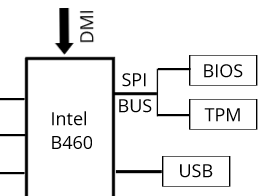
\includegraphics[width=0.8\linewidth]{SPI}
	\caption{Mainboard Blockdiagramm \cite{GIGABYTETECHNOLOGYCO.LTD.}}
	\label{fig:SPI}
\end{figure}

Aus Kostengründen ist es üblich mehrere SPI-fähige Chips, die als Slave agieren, auf den gleichen Bus zugreifen zu lassen. Ein Logik Analyzer, der einen 10-24 MHz Schiebetakt unterstützt und mindestens vier Signale gleichzeitig aufzeichnen kann, ist in der Lage die gesamte Master-Slave-Kommunikation abzufangen.
Die Beschriftung des Mainboards verrät, dass es sich bei dem BIOS Chip um das Modell MXIC MX 25L6406E M2I-12G mit der Bauform SOIC-8 handelt. Der Hersteller stellt auch hier ein Schema der Pins bereit.

\begin{figure}[h!]
	\centering
	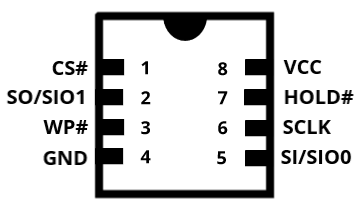
\includegraphics[width=0.9\linewidth]{BIOS}
	\caption{MXIC BIOS \cite{MacronixInternationalCo.LTD..2010}}
	\label{fig:bios}
\end{figure}

Mit diesem Wissen können die Clips des Logik Analyzer an dem Chip angebracht, und die richtigen Channels in der dazugehörigen High Level Analyzer Software eingestellt werden.

\begin{figure}[h!]
	\centering
	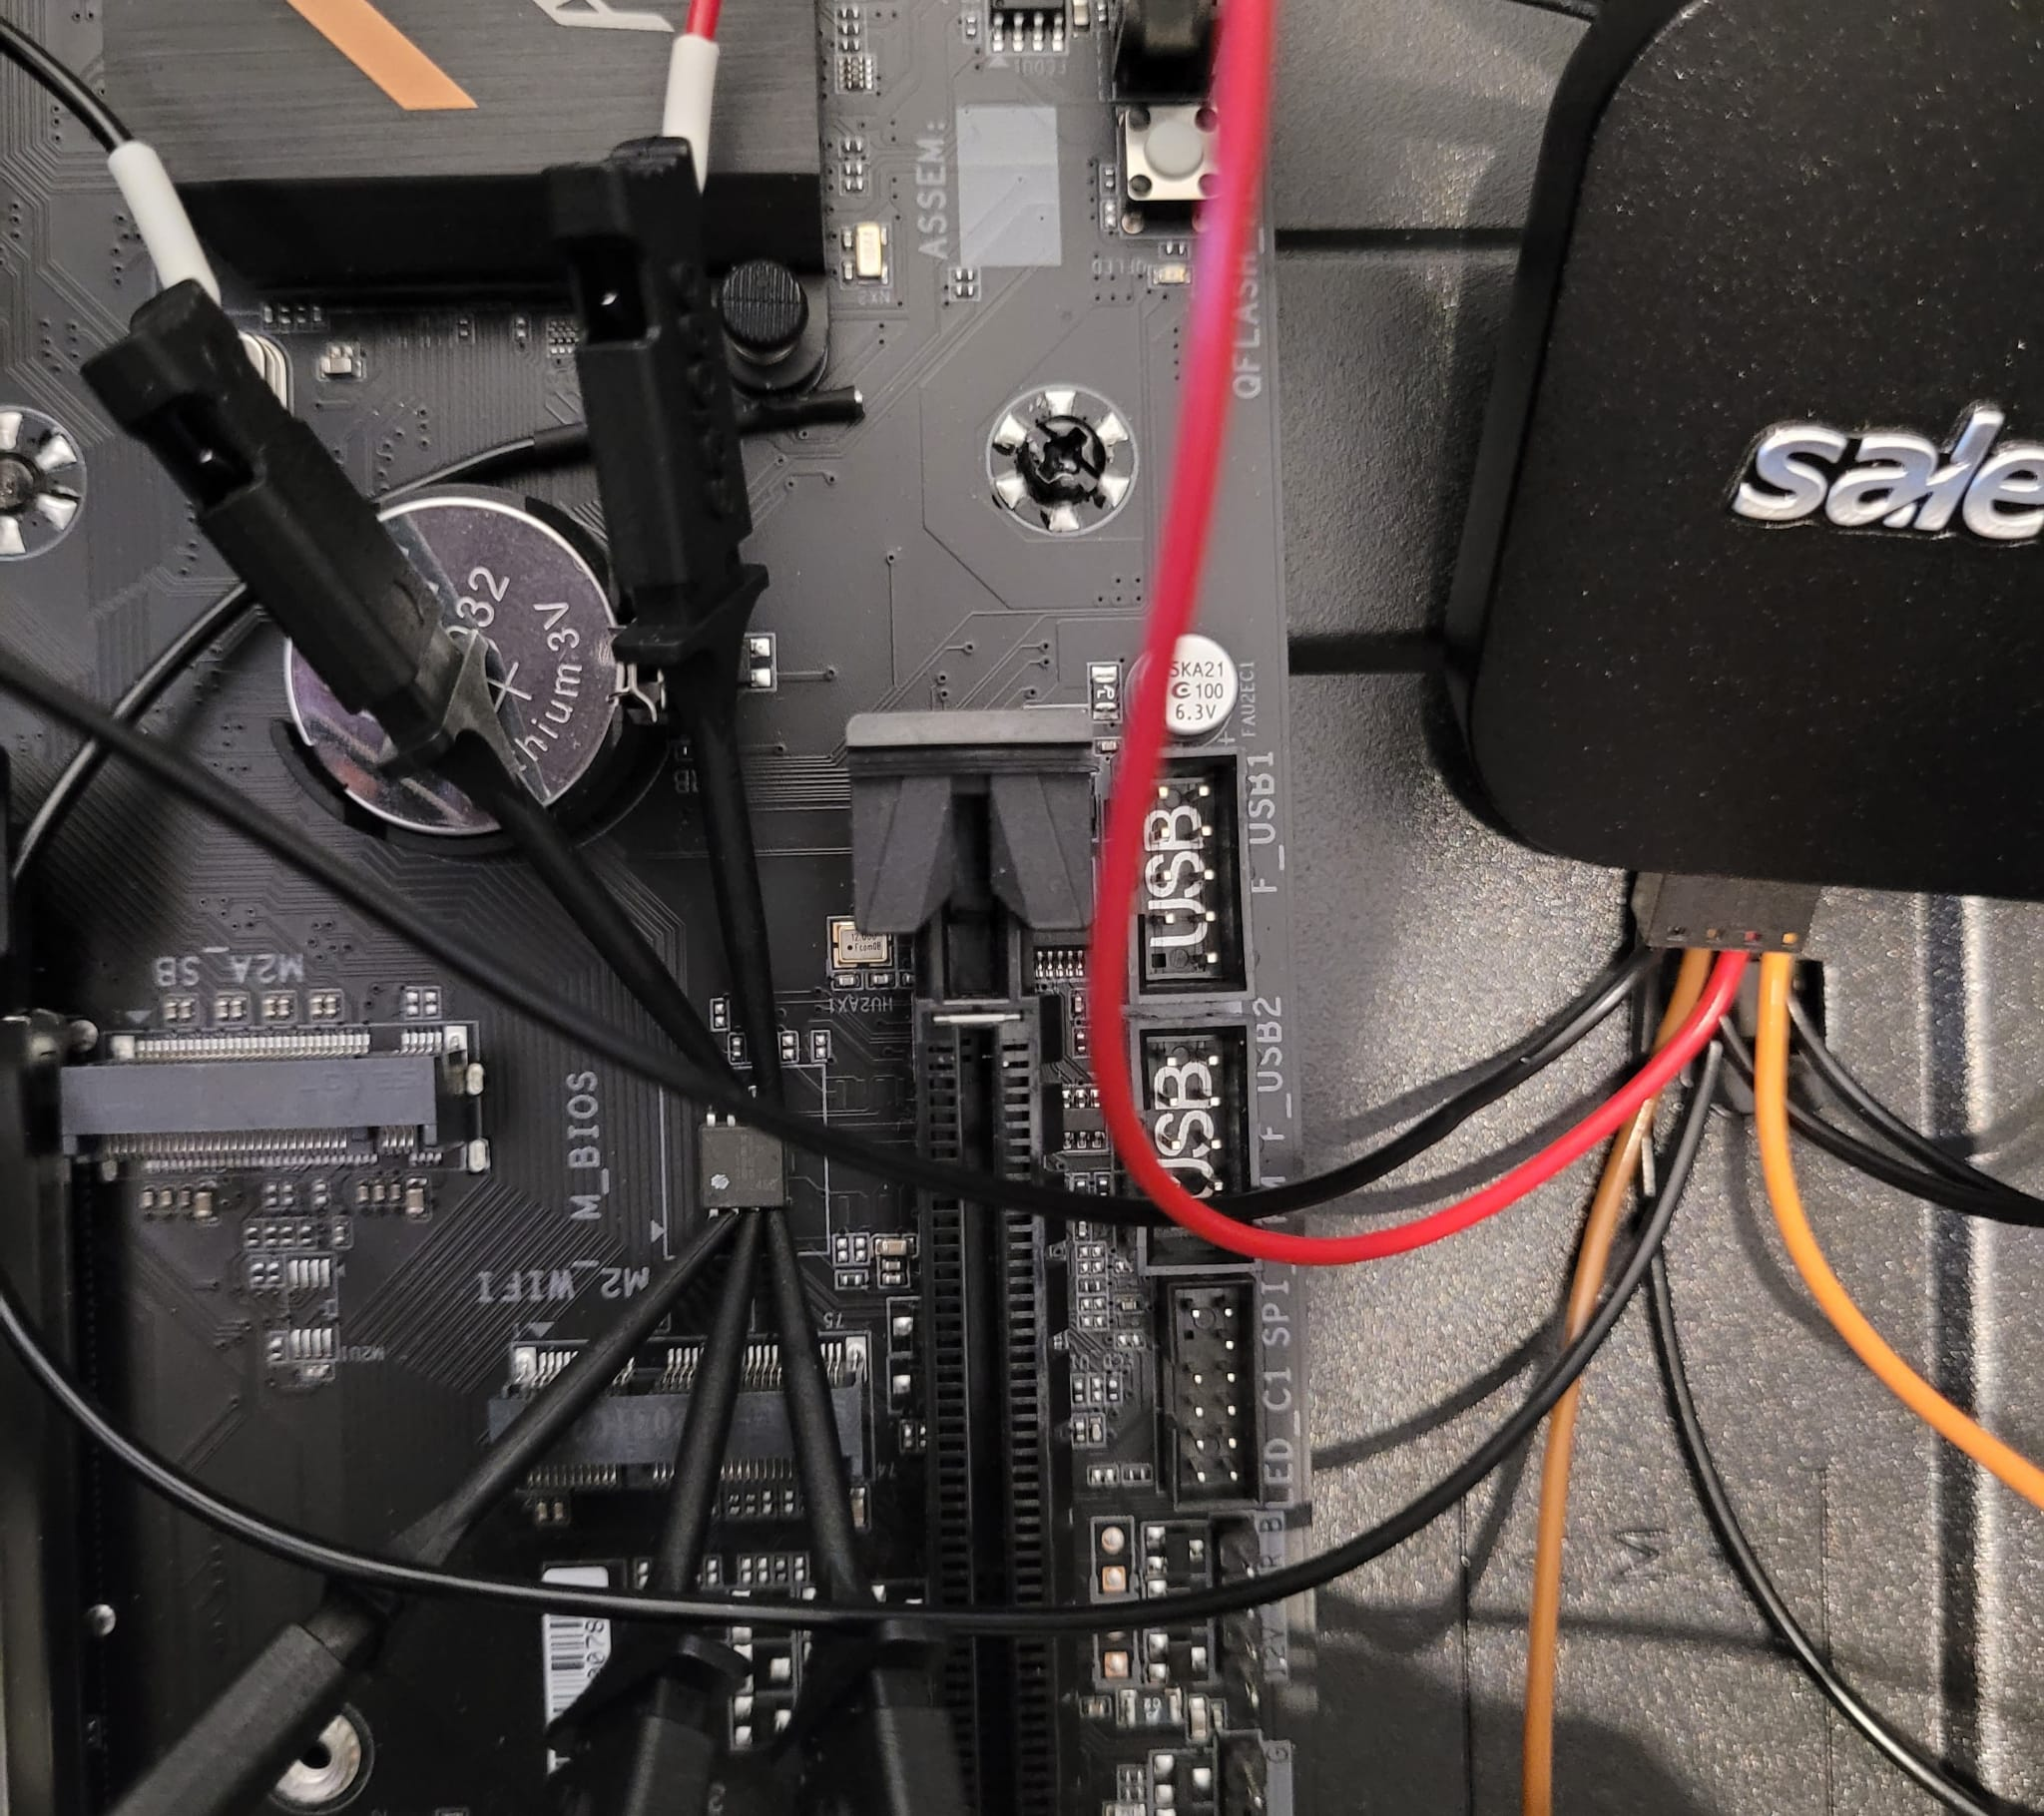
\includegraphics[width=1\linewidth]{Salea}
	\caption{Saleae Logik Analyzer}
	\label{fig:saleae}
\end{figure}

\subsection{Extrahieren des BitLocker-Schlüssels}
Nach dem Abfangen der Daten wird das Capture in einen High Level Analyzer geladen. Für den Versuch wird Logic Pro 16 genutzt, die hauseigenen Software des Saleae Logik Analyzers \cite{.13122021}. Um zu validieren, dass beim Abhören keine Fehler unterlaufen sind, wird ein SPI Analyzer ausgewählt und der Channel der jeweiligen SPI-Leitung nach Tabelle \ref{tab:Analyzer} zugewiesen. Wenn alle Werte in einem gültigen Hexadezimalbereich liegen und der Analyzer die Daten des Enable Channels auslesen kann, handelt es sich um valide SPI-Kommunikationsdaten. \pagebreak

\begin{figure}[h!]
	\centering
	\begin{tabular}{| l | l |}
		\hline
		Channel & SPI Leitung \\
		\hline
		1 & Enable \\	
		\hline
		2 & MOSI \\
		\hline
		3 & MISO \\
		\hline
		4 & Clock \\
		\hline
	\end{tabular}
	\caption{SPI Analyzer}
	\label{tab:Analyzer}
\end{figure}

Zum Finden des BitLocker Schlüssels gibt es bereits ein von Henri Numri entwickeltes Toolkit \cite{GitHub.14122021}. Es umfasst die Funktionalität, den Datenfluss des TPMs über SPI zu decodieren, sowie die Möglichkeit den BitLocker-Schlüssel direkt zu extrahieren. Nach der Installation der Erweiterung kann diese als Analyzer ``BitLocker Key Extractor'' ausgewählt und die Analyse gestartet werden. Nach ein paar Minuten wird der gefundene BitLocker Recovery Schlüssel im Datenfeld ausgegeben.

\begin{figure}[h!]
	\centering
	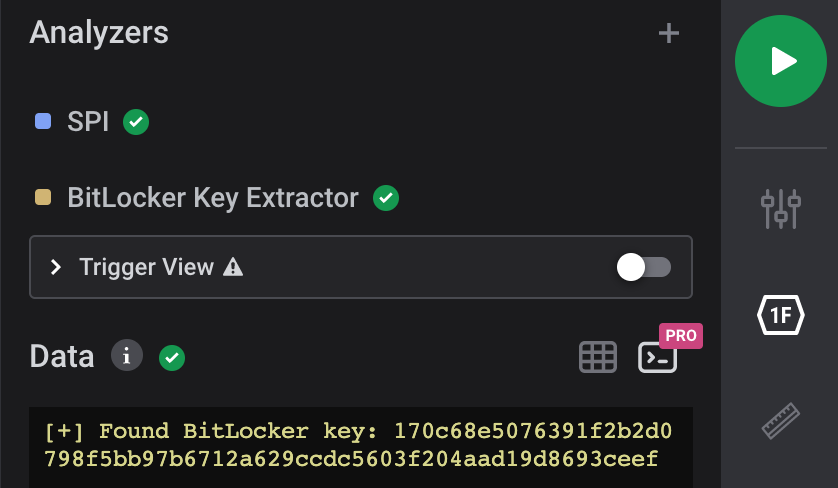
\includegraphics[width=0.8\linewidth]{LogicPro}
	\caption{High-Level Analyzer \cite{GitHub.14122021}}
	\label{fig:LogikPro}
\end{figure}

Nun kann die mit BitLocker verschlüsselte Festplatte ausgebaut und mit dem entsprechenden Adapter an unser Angreifersystem angeschlossen werden. Zum Entschlüsseln wird die ``dislocker-file'' Funktion der Open Source Software Dislocker \cite{GitHub.14122021b} verwendet. Durch den Befehl in Abbildung \ref{fig:Dislocker} wird die verschlüsselte Partition in eine flatfile Datei entschlüsselt und als NTFS-Partition formatiert, welche direkten Klartextzugriff erlaubt.

\begin{figure}[h!]
	\begin{lstlisting}
dislocker-file [-hqrsv] [-l LOG_FILE] 
[-O OFFSET] [-V VOLUME DECRYPTMETHOD -F[N]] 
[--] NTFS_FILE
	\end{lstlisting}
	\caption{Dislocker}
	\label{fig:Dislocker}
\end{figure}

\section{Evaluation}
Nachdem die Durchführbarkeit des Angriffs bewiesen wurde, wird hier noch einmal die realistische Umsetzbarkeit anhand von verschiedenen Faktoren überprüft.

\begin{itemize}
	
	\item {\bf Zeit:} Der initiale Versuch war mit einem Zeitaufwand von 4 Stunden verbunden. Der größte Anteil ist der Anpassung an den spezifischen TPM zuzuschreiben. Ein zweiter Durchlauf des Angriffs konnte in unter 15 Minuten durchgeführt werden. 
	\item {\bf Ressourcen:} Zur Durchführung wird eine Logik Analyzer mit den entsprechenden Kabeln und Clips, Schraubenzieher sowie ein Computer/Laptop benötigt. 
	\item {\bf Kosten:} Ein Logik Analyzer der den technischen Ansprüchen genüge trägt, kann bereits für 200 € erworben werden. Zusammen mit den Kosten für einen Schraubenzieher und einem System zur technischen Auswertung der Daten kann der Angriff mit einem minimalen Preis von 400 € durchgeführt werden. 
	\item {\bf Schwierigkeit:} Die größte technische Herausforderung in diesem Szenario ist das Anbringen der Testclips des Logik Analyzers an die korrekten Pins des TPM Chips. Hierfür wird das Basiswissen vorausgesetzt den Bauplan der Chips und des Mainboards lesen und verstehen zu können. Wird der Angriff entsprechend vorbereitet und die Position der anzubringenden Clips dokumentiert, kann dies auch durch einen Laien durchgeführt werden.
	\item {\bf Benutzerverifikation:} Solange der BitLocker die Standardmäßig von Windows vorgegebenen Einstellungen, BitLocker mit TPM ohne Pin oder Hardwaretoken, nutzt kann der BitLocker Schlüssel ausgelesen werden.
	
\end{itemize}

\section{Fazit}
Wie an dem Versuchsaufbau gezeigt, kann der Schutz durch Festplattenverschlüsselung in Kombination mit einem TPM umgangen werden. Im Gegensatz zu bereits etablieren Verfahren ist das Auslesen des BitLocker-Schlüssels eine schnelle, durch den Logik Analyzer jedoch auch kostspieligere Methode. Die initiale Durchführung fordert einen größeren Zeit- und Wissensaufwand, kann dann jedoch einfach reproduziert werden. Auch ist die Durchführung nicht an jedem Gerät möglich, der TPM oder auf dem SPI-Bus liegende Chips müssen ausreichend groß und während des Bootvorganges erreichbar sein. Des Weiteren können Angriffe dieser Art einfach durch die Einführung einer zusätzlichen Benutzerauthentifizierung vorgebeugt werden. BitLocker stellt hierfür unterschiedliche Möglichkeiten bereit, beispielsweise durch einen Hardwaretoken, meist in Form eines speziellen USB-Sticks oder durch einen vom Benutzer festgelegten PIN. 

\section{Literatur}
% Binden die TPM.bib mit ein
\printbibliography[heading=none]

\end{document}


